\chapter{Dispersión estelar y base de datos GAIA}
\label{chap:dispersion}
Este capítulo presenta los fundamentos necesarios para el estudio de la dispersión estelar en la Vía Láctea.
Se describe la base de datos GAIA DR3, utilizada como fuente principal de información astrométrica y física, y se detallan los parámetros seleccionados para el análisis.
A continuación, se explican los cálculos realizados para transformar los datos observacionales en magnitudes físicas.
Finalmente, se presenta el marco físico y computacional utilizado para calcular la dispersión estelar, incluyendo el esquema de integración temporal y el tratamiento de las interacciones gravitatorias entre estrellas.

\section{Base de datos GAIA}\label{sec:GAIA}

La misión \textbf{GAIA} de la Agencia Espacial Europea (ESA) es uno de los proyectos más ambiciosos de la astronomía moderna~\cite{gaia_mission_esa}.
Su objetivo principal es realizar un censo y un mapa tridimensional cosmológico lo más preciso y completo de las estrellas de la Vía Láctea.
Además de estrellas, también recolecta información acerca de: cúmulos estelares, cúmulos globulares, galaxias externas y cuásares.
Toda esta información proviene del satélite del mismo nombre que se muestra en la figura~\ref{fig:sonda}.

Lanzado el 19 de diciembre de 2013 desde la Guyana Francesa, el satélite Gaia se posicionó en una órbita alrededor del Sol a 1,5 millones de km de la Tierra en un espacio conocido como punto de Lagrange L2.
Este es un espacio privilegiado para realizar observaciones, ya que las fuerzas gravitacionales del Sol y la Tierra se equilibran con la fuerza centrífuga del satélite, por lo que sería la posición final de la sonda durante toda la duración de la misión.
La duración prevista de la misión era de 5 años, pero debido al excelente rendimiento y estabilidad que presenta, ha sido extendida en varias ocasiones y continúa activa en la actualidad.

La sonda envía datos brutos periódicamente a la Tierra que son procesados y, cada cierto tiempo, transformados en catálogos públicos conocidos como \textbf{Data Releases (DR)}.
Estos Data Release se publican de forma progresiva a través del \textbf{Gaia Archive}~\cite{gaia_archive}.
Hasta la fecha, se han publicado varios lanzamientos importantes (DR1 en 2016, DR2 en 2018 y EDR3/DR3 en 2020–2022), cada uno de ellos con mejoras sustanciales en precisión y volumen de datos.
El próximo lanzamiento, \textbf{Gaia DR4}, se encuentra actualmente en fase de preparación y se espera su publicación en diciembre de 2026.

En la siguiente subsección se profundizará en la estructura y el contenido del Data Release 3 utilizado en este proyecto.

\begin{figure}[hp!]
    \centering
    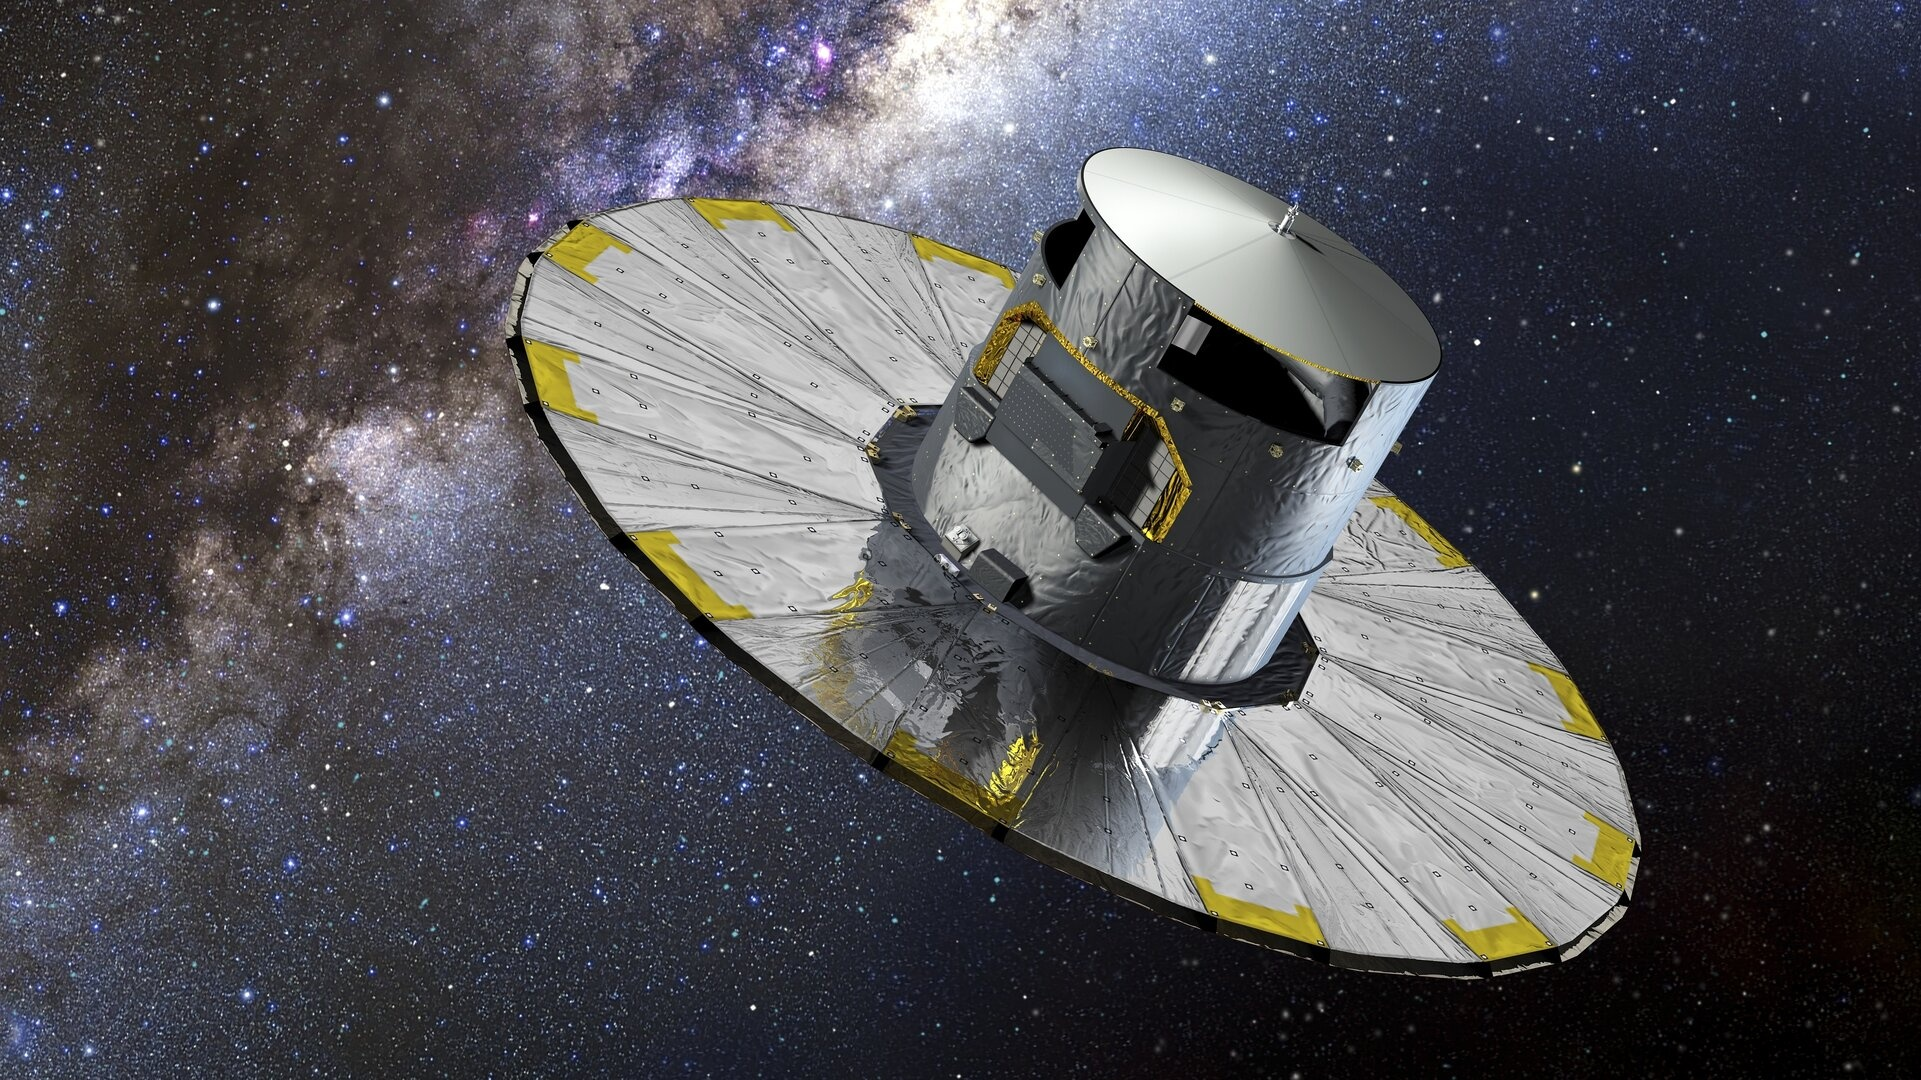
\includegraphics[width=\textwidth]{imaxes/gaia}
    \caption{Representación de la sonda Gaia}
    \label{fig:sonda}
\end{figure}

\subsection{Composición y estructura de los datos}\label{subsec:composicion}
El \textbf{Data Release 3 (DR3)}~\cite{gaia_dr3_documentation} de la misión Gaia constituye el conjunto de datos más completo y preciso publicado hasta la fecha por la ESA\@.
Fue presentado oficialmente el 13 de junio de 2022 e incluye observaciones recopiladas durante los primeros 34 meses de operación científica del satélite, entre julio de 2014 y mayo de 2017.
Este lanzamiento representa un avance sustancial respecto a los catálogos anteriores (DR1 y DR2), tanto en el número de estrellas registradas como en la calidad y variedad de los parámetros disponibles.

El catálogo contiene información astrométrica, fotométrica y espectroscópica de más de \textbf{1.800 millones de objetos}, de los cuales aproximadamente 1.500 millones poseen soluciones astrométricas completas, es decir, posición, paralaje(desplazamiento con respecto a las demás estrellas) y movimiento propio.
Esta información se almacena en distintas tablas temáticas.
A continuación se detallan las más relevantes y necesarias para este proyecto.
Cada fila de estas tablas representa un único objeto observado al que se asocia a un identificador numérico \texttt{source\_id} que permite identificarlo y cruzarlo con distintas tablas y catálogos.
\subsubsection{Tabla \texttt{gaia\_source}}
La tabla \texttt{gaia\_source} contiene los parámetros fundamentales de cada objeto observado.
Esta tabla contiene más de cien columnas y constituye la base de las demás tablas, pero para la realización de este proyecto solo son necesarias 9 de sus columnas:
\begin{itemize}
    \item \texttt{source\_id}: Identificador común mencionado anteriormente.
    Está construido mediante el sistema de indexación jerárquico HEALPix\footnote{HEALPix. Disponible en: \url{https://healpix.sourceforge.io/}{HEALPix - Features}}, lo que permite conocer la localización aproximada de la estrella en el cielo.
    Este identificador es único para cada fuente y se utiliza para realizar referencias cruzadas entre las distintas tablas del archivo Gaia y otras bases de datos astronómicas.

    \item \texttt{ra}($\alpha$): Ascensión Recta , expresada en grados y referida al sistema de coordenadas ecuatoriales (epoch J2016.0).
    \footnote{El término \textit{epoch 2016} indica la fecha de referencia para las coordenadas y los movimientos propios utilizados en el catálogo. En astronomía, las posiciones de las estrellas cambian lentamente con el tiempo debido a su movimiento real en el espacio y a efectos como la precesión. Por ello, los catálogos fijan una \textit{época} (en este caso el año 2016) como punto de referencia a partir del cual se definen y extrapolan las posiciones estelares.}
    Indica la posición de la fuente en el eje Este–Oeste del cielo y, junto con la declinación, determina su ubicación precisa en la bóveda celeste.

    \item \texttt{dec}($\delta$): Declinación , también en grados, medida en el sistema ecuatorial.
    Representa la posición angular de la fuente respecto al ecuador celeste, análoga a la latitud terrestre.
    Combinada con \texttt{ra}, define la posición bidimensional de la fuente observada.

    \item \texttt{pmra}: Movimiento propio en dirección de ascensión recta ($\mu_{\alpha}\cos\delta$), expresado en milisegundos de arco por año (mas/yr).
    Incluye el factor $\cos(\delta)$ para corregir la convergencia de meridianos hacia los polos.
    Indica el desplazamiento aparente de la fuente a lo largo del eje de ascensión recta debido a su movimiento real dentro de la galaxia.

    \item \texttt{pmdec}: Movimiento propio en dirección de declinación ($\mu_{\delta}$), también en mas/yr.
    Describe el desplazamiento aparente de la estrella en el eje Norte–Sur del cielo.
    Combinando \texttt{pmra} y \texttt{pmdec} puede calcularse la velocidad tangencial proyectada de la fuente, información esencial para el estudio cinemático de la Vía Láctea.

    \item \texttt{radial\_velocity}: Velocidad radial de la estrella respecto al Sol, expresada en km/s.
    Este parámetro se obtiene a partir del \textit{Radial Velocity Spectrometer} (RVS) a bordo de Gaia.
    Permite conocer el componente de la velocidad en la línea de visión y, junto con los movimientos propios, reconstruir el vector de movimiento tridimensional de la fuente.

    \item \texttt{phot\_g\_mean\_mag}: Magnitud aparente media en la banda fotométrica \texttt{G}, calibrada en el sistema Vega, es una medida directa del brillo observado.
    Este valor, combinado con la distancia, permite calcular la magnitud absoluta y, por tanto, la luminosidad estelar.

    \item \texttt{bp\_rp}: Color fotométrico definido como la diferencia entre las magnitudes medias en las bandas azul (\texttt{BP}) y roja (\texttt{RP}).
    Este índice de color es un indicador directo de la temperatura efectiva de la estrella.

    \item \texttt{logg\_gspphot}: Logaritmo de la gravedad superficial de la estrella, expresado en cm/s$^2$ y estimado por el módulo fotométrico \texttt{GSP-Phot}.
    Valores altos corresponden a estrellas de la secuencia principal, mientras que valores bajos son típicos de gigantes o supergigantes.
\end{itemize}
\subsubsection{Tabla \texttt{astrophysical\_parameters}}
Las columnas extraídas de la tabla \texttt{astrophysical\_parameters} pertenecen al módulo \texttt{FLAME} (\textit{Final Luminosity, Age and Mass Estimator}), encargado de estimar parámetros físicos de las estrellas a partir de la información fotométrica y de modelos de evolución estelar.
A continuación se describen las columnas empleadas en este trabajo:

\begin{itemize}
    \item \texttt{source\_id}: Identificador único de la fuente, común con la tabla \texttt{gaia\_source}.
    Es la clave primaria utilizada en las consultas cruzadas entre tablas.

    \item \texttt{mass\_flame}: Masa estelar estimada en unidades de masa solar ($M_{\odot}$). Este valor se obtiene mediante el ajuste de modelos teóricos de evolución estelar a las observaciones fotométricas y astrométricas (paralaje, temperatura efectiva, luminosidad y metalicidad).

    \item \texttt{radius\_flame}: Radio estelar estimado en unidades de radio solar ($R_{\odot}$), derivado de los mismos modelos empleados por el módulo \texttt{FLAME}.
    Este parámetro indica el tamaño físico aproximado de la estrella.
    En combinación con la temperatura efectiva y la luminosidad, permite situar la estrella dentro del diagrama de Hertzsprung–Russell\footnote{Más información disponible en: \url{https://es.wikipedia.org/wiki/Diagrama_de_Hertzsprung-Russell}} y estimar su estado evolutivo (secuencia principal, subgigante o gigante).
\end{itemize}
\subsubsection{Parámetro adicional}
Además de las columnas anteriores, se incluye también el parámetro \texttt{rgeo}, obtenido a través del servicio \textit{TAP VizieR}\footnote{TAP VizieR. Disponible en: \url{https://tapvizier.u-strasbg.fr/adql/}}, que proporciona datos complementarios derivados de catálogos externos al archivo principal de Gaia:

\begin{itemize}
    \item \texttt{rgeo}: Distancia geométrica estimada en parsecs (pc)\footnote{1 pc equivale a 3.26 años luz o 3,0857 \times 10^{13}km} basada en el método bayesiano desarrollado por Bailer-Jones~\cite{Bailer-Jones2021}.
    Este parámetro corrige las incertidumbres y sesgos asociados al cálculo directo de la distancia mediante la inversa del paralaje, especialmente relevantes en regiones con errores elevados o valores negativos de paralaje.
    El valor de \texttt{rgeo} representa la mejor estimación estadística de la distancia a la fuente, teniendo en cuenta tanto la medida observacional como un modelo de distribución espacial de estrellas en la galaxia.
    Resulta fundamental para convertir magnitudes aparentes en magnitudes absolutas y para estimar luminosidades físicas de las estrellas con mayor precisión.
\end{itemize}

\section{Selección y filtrado de los datos}\label{sec:filtrado}
El catálogo \textbf{Gaia DR3} contiene información astrométrica, fotométrica y espectroscópica de más de \textbf{1.800 millones de fuentes}.
Sin embargo, para los objetivos de este trabajo no todas las fuentes son adecuadas, ya que poblaciones evolucionadas (gigantes, subgigantes o enanas blancas) presentan cinemáticas y distribuciones espaciales distintas, lo que impide calcular adecuadamente algunos de sus parámetros.

Por esta razón, se selecciona únicamente la población de \textbf{estrellas de la secuencia principal}, definida en el diagrama color–magnitud por el intervalo fotométrico:

\[
    0.3 < (BP - RP) < 2.0.
\]

Esta restricción garantiza que las estrellas analizadas se encuentren en una fase estable de evolución estelar, dominada por la fusión de hidrógeno en el núcleo.

Adicionalmente, se descartan todas las fuentes con información incompleta, es decir, aquellas que presentan valores nulos (\texttt{NULL}) en alguna de las siguientes columnas esenciales:
\texttt{bp\_rp}, \texttt{phot\_g\_mean\_mag} o \texttt{rgeo}.
Este filtrado no solo garantiza la coherencia de las magnitudes físicas calculadas, sino que también reduce el tamaño efectivo del conjunto de datos, lo cual es crucial desde el punto de vista computacional.

Tras aplicar ambos criterios, la restricción fotométrica de secuencia principal y la eliminación de registros incompletos, la muestra final empleada en este trabajo queda compuesta por \textbf{1.174.075.109 estrellas}.

\section{Transformación de los datos}\label{sec:calculos_previos}

Para poder computar la dispersión estelar necesitamos caracterizar completamente la posición, el movimiento y las propiedades fundamentales de cada estrella utilizando un sistema de referencia coherente.
En esta sección describimos cómo transformamos los datos disponibles en el catálogo Gaia DR3 para obtener las magnitudes físicas  y espaciales que vamos a necesitar.
\subsection{Transformación de coordenadas}\label{subsec:transformacion-de-coordenadas}

Las coordenadas ecuatoriales $(\alpha, \delta)$ describen la posición de una estrella en la esfera celeste tomando como referencia el ecuador terrestre proyectado en el cielo.
No obstante, para estudiar la estructura y dinámica de la Vía Láctea resulta más útil emplear un sistema de referencia ligado a su propio plano.
Este sistema es el de \textbf{coordenadas galácticas}, en el cual las posiciones se expresan respecto al centro de la galaxia.

En este sistema:
\begin{itemize}
    \item El \textbf{origen} se sitúa en el \textbf{centro galáctico}.
    \item El eje $X$ apunta hacia el \textbf{centro galáctico} (dirección de la constelación de Sagitario).
    \item El eje $Z$ apunta hacia el \textbf{polo norte galáctico}, perpendicular al plano galáctico.
    \item El eje $Y$ completa el sistema formando una base dextrógira (regla de la mano derecha).
\end{itemize}

La conversión entre coordenadas ecuatoriales y galácticas puede expresarse como una rotación en el espacio tridimensional.
La orientación del plano galáctico fue definida por la IAU, y la matriz de rotación asociada es:

\[
    \mathbf{R} =
    \begin{bmatrix}
        -0.05487556 & -0.87343709 & -0.48383502 \\
        +0.49410943 & -0.44482963 & +0.74698225 \\
        -0.86766615 & -0.19807637 & +0.45598380
    \end{bmatrix},
\]

cuyas constantes fueron establecidas por Murray (1989) y continúan siendo el estándar actual en herramientas astrométricas modernas como \texttt{Astropy}~\cite{murray1989_coordinates}.
Dado que el sistema de referencia de Gaia DR3 está alineado con el ICRS (Sistema de Referencia Celeste Internacional), esta matriz es directamente aplicable a los datos utilizados en este trabajo.

Para una estrella situada a una distancia heliocéntrica $d$ (en parsecs), se construye primero el vector de posición unitario en el sistema ecuatorial:

\[
    \hat{\mathbf{r}}_E =
    \begin{pmatrix}
        \cos \delta \cos \alpha \\
        \cos \delta \sin \alpha \\
        \sin \delta
    \end{pmatrix}
\]

Al multiplicarlo por la matriz $\mathbf{R}$ obtenemos la dirección en el sistema galáctico, y al escalar por $d/1000$ expresamos la posición en kiloparsecs:

\[
    \begin{pmatrix}
        X \\ Y \\ Z
    \end{pmatrix}
    =
    \frac{d}{1000}\,
    \mathbf{R}\,
    \hat{\mathbf{r}}_E
\]

Esta transformación permite situar la estrella en un sistema de referencia coherente con la geometría de la Vía Láctea, lo cual es fundamental para el análisis de su estructura y distribución espacial.

\subsection{Estimación de la Velocidad Radial}\label{subsec:estimacion-de-la-velocidad-radial}
La velocidad radial \( v_r \) representa la componente de la velocidad estelar proyectada a lo largo de la línea de visión del observador.
En caso de no estar disponible en el catálogo para una determinada estrella, se realiza una estimación basada en su posición y movimientos propios, aplicando la formulación clásica de Johnson \& Soderblom~\cite{johnson1987}.


El punto de partida son los movimientos propios en ascensión recta y declinación (\( \mu_{\alpha} \)) y (\( \mu_{\delta} \)), los cuales describen cómo cambia la posición aparente de la estrella en la esfera celeste.
Estos movimientos propios corresponden únicamente a la componente tangencial de la velocidad estelar, es decir, perpendicular a la línea de visión.
Para convertirlos en una velocidad física en el espacio, es necesario combinarlos con la distancia \( d \) a la estrella.

Primero, calculamos la velocidad tangencial tridimensional.
Para ello se utiliza una matriz de transformación \( T \) , que permite transformar las variaciones angulares observadas sobre la esfera celeste en componentes cartesianas en un sistema de coordenadas ecuatoriales:
\[
    T =
    \begin{pmatrix}
        -\sin\alpha & -\cos\alpha \sin\delta \\
        \cos\alpha & -\sin\alpha \sin\delta \\
        0 & \cos\delta
    \end{pmatrix}
\]

donde \(\alpha\) y \(\delta\) son la ascensión recta y la declinación de la estrella.
La velocidad tangencial resultante se obtiene como:

\[
    \vec{V} = \kappa \, d \,
    T
    \begin{pmatrix}
        \mu_{\alpha} \\
        \mu_{\delta}
    \end{pmatrix}
\]

donde \(\kappa = 4.74047\) es el factor de conversión entre movimiento propio (en mas/año), distancia (en parsecs) y velocidad (en km/s).

Posteriormente, la proyección de este vector sobre la dirección de la línea de visión (definida por las coordenadas galactocéntricas \( C_x, C_y, C_z \)) proporciona una primera estimación de la componente radial.
\[
    V_{\text{radial\_sin}} =
    \frac{C_x V_x + C_y V_y + C_z V_z}
    {\sqrt{C_x^2 + C_y^2 + C_z^2}}
\]
A esta estimación se le añaden dos correcciones:

\begin{enumerate}
    \item \textbf{Corrección por rotación galáctica}, calculada como:
    \[
        V_{\text{rot}} = V_{\text{GAL}} \frac{C_y}{\sqrt{C_x^2 + C_y^2}}
    \]
    donde \( V_{\text{GAL}} \) es la velocidad de rotación del Sol alrededor del centro galáctico.

    \item \textbf{Corrección por el movimiento peculiar del Sol}, determinada mediante:
    \[
        V_{\text{sol}} = \frac{U_{\text{SOL}} C_x + V_{\text{SOL}} C_y + W_{\text{SOL}} C_z}{\sqrt{C_x^2 + C_y^2 + C_z^2}}
    \]
    donde \( (U_{\text{SOL}}, V_{\text{SOL}}, W_{\text{SOL}}) \) representan las componentes de la velocidad solar respecto al entorno local.
\end{enumerate}

Finalmente, la velocidad radial estimada se obtiene como:

\[
    v_r = V_{\text{radial\_sin}} + V_{\text{rot}} - V_{\text{sol}}
\]
En este trabajo se adoptan los valores propuestos por Schönrich et al\cite{schonrich2010,blandhawthorn2016} para el movimiento solar:
\( V_{\text{GAL}} = 220~\text{km s}^{-1} \), \( U_{\text{SOL}} = 11.1~\text{km s}^{-1}\), \( V_{\text{SOL}} = 12.24~\text{km s}^{-1}\), \( W_{\text{SOL}} = 7.25~\text{km s}^{-1}\).

De este modo, el procedimiento permite aproximar la velocidad radial de una estrella a partir de parámetros astrométricos disponibles (posición, movimientos propios y distancia), incluyendo los efectos de la rotación galáctica y del movimiento solar.
\subsection{Cálculo de las velocidades espaciales}\label{subsec:calculo-de-las-velocidades-espaciales}

A través de los movimientos propios observados en ascensión recta y declinación, \(\mu_{\alpha}\cos\delta\) y \(\mu_{\delta}\) (expresados en mas\,año\(^{-1}\)), junto con una distancia \(d\) (en parsec) y una velocidad radial observada \(V_r\) (en km\,s\(^{-1}\)), es posible determinar las componentes de la velocidad espacial en el sistema galáctico \((V_X, V_Y, V_Z)\).

El cálculo se basa en la conversión de las magnitudes observadas (coordenadas ecuatoriales) al sistema cartesiano galáctico utilizando de nuevo la formulación de Johnson \& Soderblom~\cite{johnson1987}.
Primero se obtiene la velocidad tangencial en las direcciones de ascensión recta y declinación mediante:
\[
    V_{t,\alpha} = \kappa \, d \, \mu_{\alpha}\cos\delta,
    \qquad
    V_{t,\delta} = \kappa \, d \, \mu_{\delta},
\]

donde \(\kappa = 4.74047\) es el factor de conversión que relaciona movimientos propios (mas\,año\(^{-1}\)) y distancias (pc) con velocidades en km\,s\(^{-1}\).

A partir de la velocidad radial \(V_r\) y de las velocidades tangenciales \(V_{t,\alpha}\) y \(V_{t,\delta}\),
se calcula el vector velocidad en el sistema ecuatorial:

\[
    \vec{V}_E' = V_r\,\hat{\mathbf{r}}_E + T
    \begin{pmatrix}
        V_{t,\alpha} \\
        V_{t,\delta}
    \end{pmatrix}
\]

donde \(\hat{\mathbf{r}}_E\) es el vector unitario que apunta hacia la estrella en coordenadas ecuatoriales,
y \(T\) es la matriz que proyecta las velocidades tangenciales sobre el sistema cartesiano ecuatorial definidas con anterioridad.

Finalmente, para obtener las componentes de velocidad en el sistema de referencia galáctico,
se aplica una rotación mediante la matriz \(R\) vista anteriormente, que transforma las coordenadas ecuatoriales al sistema galáctico:

\[
    \begin{pmatrix}
        V_X \\
        V_Y \\
        V_Z
    \end{pmatrix}
    =
    R \cdot
    \vec{V}_E'
    \cdot \Sigma,
\]

donde \(\Sigma = 0.0010227\) es el factor de conversión de km\,s\(^{-1}\) a kiloparsec por millón de años (kpc\,Myr\(^{-1}\)).

De este modo, se obtienen las componentes \((V_X, V_Y, V_Z)\) en el sistema galáctico,
que describen el movimiento tridimensional de la estrella respecto al centro galáctico,
expresadas en unidades de kiloparsecs por millón de años (kpc\,Myr\(^{-1}\)).
\subsection{Estimación de masas estelares}\label{subsec:estimacion-de-masas-estelares}

Para las estrellas con parámetros atmosféricos conocidos, la masa se estima a partir de la relación entre la gravedad superficial $g$ y el radio estelar $R$~\cite{carroll2017}:

\[
    \log_{10}\left(\frac{M}{M_\odot}\right) = \log g - \log g_\odot + 2 \log_{10}\left(\frac{R}{R_\odot}\right)
\]

donde $\log g_\odot = 4.437$ es el valor adoptado para el Sol.
En los casos en los que la estimación directa no es posible, se aplica una relación empírica entre la masa, el color fotométrico $(BP-RP)$ y la magnitud absoluta $M_G$, siguiendo la metodología del módulo FLAME de Gaia DR3~\cite{gaia_dr3_flame}:

\[
    \log_{10}\left(\frac{M}{M_\odot}\right) = a \,(BP-RP) + b \, M_G + c
\]

con coeficientes ajustados para estrellas de la secuencia principal solar–metalicidad:
$a = -0.15$, $b = -0.10$, $c = 1.2$.
Esta aproximación permite mantener la coherencia de los datos incluso para fuentes incompletas, proporcionando una estimación razonable de la masa estelar en ausencia de mediciones directas.
\bigskip

Tras estos cálculos previos y las correspondientes transformaciones, se obtienen los datos necesarios en las unidades adecuadas para realizar los cálculos de dispersión estelar:

\begin{itemize}
    \item \textbf{Posición galactocéntrica} en kiloparsecs: \((C_X, C_Y, C_Z)\)
    \item \textbf{Velocidad galactocéntrica} en kiloparsecs por millón de años: \((V_X, V_Y, V_Z)\)
    \item \textbf{Masa estelar} en masas solares: \textit{mass}
\end{itemize}

\section{Cálculo de la dispersión estelar}\label{sec:dispersion}

Tras obtener las posiciones y velocidades galactocéntricas de las estrellas, el objetivo de esta sección es describir de forma detallada el marco físico y matemático empleado para calcular la dispersión estelar del sistema.
Se presentan los modelos del potencial galáctico, la forma en que se calculan las aceleraciones que rigen la dinámica del sistema y el integrador utilizado para la simulación.

\subsection{Esquema de integración temporal}\label{subsec:esquema-de-integracion-temporal-(leapfrog-kick--drift--kick).}
Para la realizar la simulación propiamente se emplea un integrador simétrico de segundo orden tipo \emph{Leapfrog} conocido como Kick--Drift--Kick~\cite{hockney1988,saha1992,springel2005}.
Este integrador realiza actualizaciones de velocidad (v) a mitad de paso y de posicion (r) a paso completo.
Denotando por \(\Delta t\) el paso temporal, las actualizaciones discretas son:
\[
    \begin{aligned}
        \mathbf{v}\!\left(t+\tfrac{\Delta t}{2}\right) &= \mathbf{v}(t) + \tfrac{\Delta t}{2}\,\mathbf{a}(t), \\[6pt]
        \mathbf{r}(t+\Delta t) &= \mathbf{r}(t) + \Delta t \,\mathbf{v}\!\left(t+\tfrac{\Delta t}{2}\right), \\[6pt]
        \mathbf{v}(t+\Delta t) &= \mathbf{v}\!\left(t+\tfrac{\Delta t}{2}\right) + \tfrac{\Delta t}{2}\,\mathbf{a}(t+\Delta t).
    \end{aligned}
\]
Este esquema es \(\mathcal{O}(\Delta t^2)\) en precisión y conserva bien las cantidades integrales (energía, momento angular) sobre escalas temporales largas, siendo por ello conveniente para simulaciones N-body de estructuras galácticas.


Para garantizar la estabilidad numérica y evitar que una estrella se desplace una distancia significativa en un solo paso de integración, el valor del paso temporal se fija de acuerdo con la velocidad máxima del sistema~\cite{dehnen2011,hockney1988}.
Sea \(v_{\max}\) la mayor velocidad galactocéntrica entre todas las estrellas y \(l_{\min}\) la escala espacial mínima resoluble.
El paso temporal máximo adoptado se calcula como
\[
    \Delta t_{\max} \;=\; \eta \, \frac{l_{\min}}{v_{\max}},
\]
donde \(\eta < 1\) es un factor de seguridad que limita el desplazamiento de cada partícula a una fracción de la resolución espacial en cada iteración.

De este modo, ninguna estrella puede recorrer una distancia superior a \(\eta\,l_{\min}\) en un único paso, lo que asegura que las aceleraciones se actualicen con suficiente frecuencia y que la integración \emph{Leapfrog Kick–Drift–Kick} conserve la energía y momento angular del sistema de forma estable.

\subsection{Aceleraciones en el sistema}\label{subsec:aceleraciones-en-el-sistema}
En cada paso del integrador, es necesario evaluar la aceleración total \(\mathbf{a}_i\) que actúa sobre cada estrella \(i\).
Esta aceleración se descompone en dos componentes principales:
\[
    \mathbf{a}_i = \mathbf{a}_{\mathrm{gal}}(\mathbf{r}_i) + \mathbf{a}_{\star-\star,i},
\]
donde \(\mathbf{a}_{\mathrm{gal}}\) es la aceleración analítica producida por el potencial galáctico fijo (halo + bulbo), y \(\mathbf{a}_{\star-\star,i}\) representa la contribución debida a las interacciones gravitatorias con las demás estrellas simuladas, lo que corresponde con el mayor coste computacional de la simulación.
\subsubsection{Aceleraciones analíticas}
\begin{itemize}
    \item \textbf{Aceleración del halo} (\(\mathbf{a}_{\mathrm{halo}}\)): representa la contribución del \emph{halo de materia oscura}, el cual domina la masa en la región externa de la galaxia.
    Se modela con un perfil NFW (Navarro–Frenk–White)~\cite{navarro1996}, cuya simetría esférica permite expresar su aceleración como función únicamente del radio galactocéntrico \(r\).
    \[
        \mathbf{a}_{\mathrm{halo}}(\mathbf{r}) = -\,\frac{G\,M_{\mathrm{enc}}(r)}{r^3}\,\mathbf{r}.
    \]
    Este término impone el campo gravitacional de gran escala, responsable de mantener la rotación galáctica aproximadamente plana.

    \item \textbf{Aceleración del bulbo} (\(\mathbf{a}_{\mathrm{bulge}}\)): describe la atracción generada por la masa concentrada en el centro galáctico.
    Se adopta el potencial de Hernquist, que reproduce la distribución de densidad de los bulbos~\cite{hernquist1990}:
    \[
        \mathbf{a}_{\mathrm{bulge}}(\mathbf{r}) = -\,\frac{G\,M_b}{r(r+a)^2}\,\mathbf{r}.
    \]
    Su efecto domina en las regiones centrales, proporcionando el confinamiento gravitatorio más intenso.
\end{itemize}
\subsubsection{Interacciones entre estrellas}
La contribución debida a las interacciones mutuas entre estrellas se obtiene a partir de la ley de gravitación de Newton.
Para dos partículas puntuales de masas \(m_i\) y \(m_j\) ubicadas en \(\mathbf{r}_i\) y \(\mathbf{r}_j\), la fuerza de atracción entre ellas será:
\[
    \mathbf{F}_{ij} \;=\; - G \, \frac{m_i m_j}{(|\mathbf{r}_i-\mathbf{r}_j|^2 + \varepsilon^2)^{3/2}} \, (\mathbf{r}_i - \mathbf{r}_j),
\]
donde \(\varepsilon\) es el parámetro de \emph{suavizado} (softening) introducido para evitar singularidades y efectos extraños en corta distancia~\cite{hockney1988}.
La aceleración sobre la partícula \(i\) por parte de \(j\) es entonces:
\[
    \mathbf{a}_{ij} \;=\; - G \, \frac{m_j}{(|\mathbf{r}_i-\mathbf{r}_j|^2 + \varepsilon^2)^{3/2}} \, (\mathbf{r}_i - \mathbf{r}_j).
\]
La aceleración de las interacciones sobre la estrella \(i\) es la suma de todas las contribuciones estelares:
\[
    \mathbf{a}_i \;=\; \sum_{j\neq i} \mathbf{a}_{ij}.
\]
Calcular exactamente la suma de las aceleraciones para todas las estrellas conduce a un coste \(O(N^2)\) lo que resulta inviable para un N grande.

Para reducir el coste computacional de la suma sobre \(j\), se puede aproximar la contribución de grupos de partículas lejanas por su masa total y centro de masa, lo que se conoce como aproximación multipolar o criterio de Barnes-Hut~\cite{barnes1986}.
Si un grupo de tamaño característico \(s\) está a distancia \(d\) del cuerpo considerado, el criterio de apertura \(\theta\) de Barnes--Hut decide si la celda puede tratarse como un único cuerpo:
\[
    \frac{s}{d} < \theta \quad \Longrightarrow \quad
    \mathbf{a}_{\text{celda}} \approx - G \, \frac{M_{\text{celda}}}{d^2} \,\hat{\mathbf{d}} .
\]
Si la desigualdad no se cumple, la celda se subdivide y se consideran sus hijos (multipolo de orden superior si se desea mayor precisión).
El parámetro \(\theta\) controla la precisión/velocidad.

